\section{归约:减少分支}
归约从值数组中派生出单个值。 单个值可以是所有元素中的总和、最大值、最小值等。 
该值还可以是各种类型:整数、单精度浮点、双精度浮点、半精度浮点、字符等。 所有这些类型的归约都具有相同的计算结构。 
与直方图一样,归约是一种重要的计算模式,因为它可以从大量数据中生成摘要。 
并行归约是一种重要的并行模式,需要并行线程相互协调才能得到正确的结果。 
这种协调必须仔细进行,以避免性能瓶颈,这在并行计算系统中很常见。 
因此,并行归约是说明这些性能瓶颈并引入缓解这些瓶颈的技术的良好工具。

\subsection{背景}
从数学上讲,如果运算符具有明确定义的标识值,则可以基于二元运算符为一组项目定义归约。 
例如,浮点加法运算符的标识值为 0.0; 也就是说,任何浮点值 v 和值 0.0 相加都会得到值 v 本身。 
因此,可以基于产生该组中所有浮点数之和的加法运算符来为一组浮点数定义归约。 
例如,对于集合 \{7.0, 2.1, 5.3, 9.0, 11.2\},求和归约将产生 $7.0+2.1 +5.3+9.0+11.2 = 34.6$。

\begin{figure}[H]
	\centering
	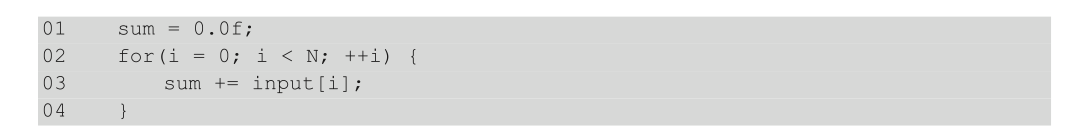
\includegraphics[width=0.9\textwidth]{figs/F10.1.png}
	\caption{\textit{一个简单的顺序求和归约代码。}}
\end{figure}

可以通过顺序遍历数组的每个元素来执行归约。 图 10.1 显示了 C 语言中的顺序求和归约代码。
该代码将结果变量 sum 初始化为恒等值 0.0。 然后,它使用 for 循环来迭代保存该组值的输入数组。 
在第 i 次迭代期间,代码对 sum 的当前值和输入数组的第 i 个元素执行加法运算。 
在我们的示例中,迭代 0 后,sum 变量包含 $0.0+7.0 = 7.0$。 迭代 1 次后,sum 变量包含 $7.0+2.1 = 9.1$。 
因此,在每次迭代之后,输入数组的另一个值将被添加(累加)到 sum 变量中。 迭代 5 次后,sum 变量包含 34.6,这是归约结果。

可以为许多其他运算符定义归约。 可以为单位值为 1.0 的浮点乘法运算符定义乘积归约。 
一组浮点数的乘积归约是所有这些数字的乘积。 可以为返回两个输入中较小值的最小比较运算符定义最小 (min) 归约。 
对于实数,最小运算符的恒等值为 $+\infty$。 可以为返回两个输入中较大值的最大 (max) 比较运算符定义最大 (max) 归约。 
对于实数,最大运算符的恒等值为 $-\infty$。

\begin{figure}[H]
	\centering
	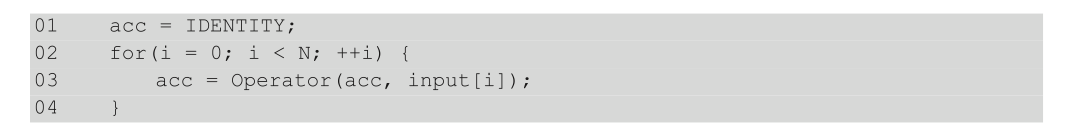
\includegraphics[width=0.9\textwidth]{figs/F10.2.png}
	\caption{\textit{顺序归约代码的一般形式。}}
\end{figure}

图 10.2 显示了运算符归约的一般形式,它被定义为接受两个输入并返回一个值的函数。 
当在 for 循环迭代期间访问某个元素时,要采取的操作取决于所执行的归约类型。 
例如,对于最大归约,运算符函数在两个输入之间执行比较并返回两个输入中的较大值。 
对于最小归约,运算符函数比较两个输入的值,并返回较小的值。 当 for 循环访问完所有元素时,顺序算法结束。 
对于一组 N 个元素,for 循环会迭代 N 次,并在循环出口处生成归约结果。

\subsection{归约树}
\begin{figure}[H]
	\centering
	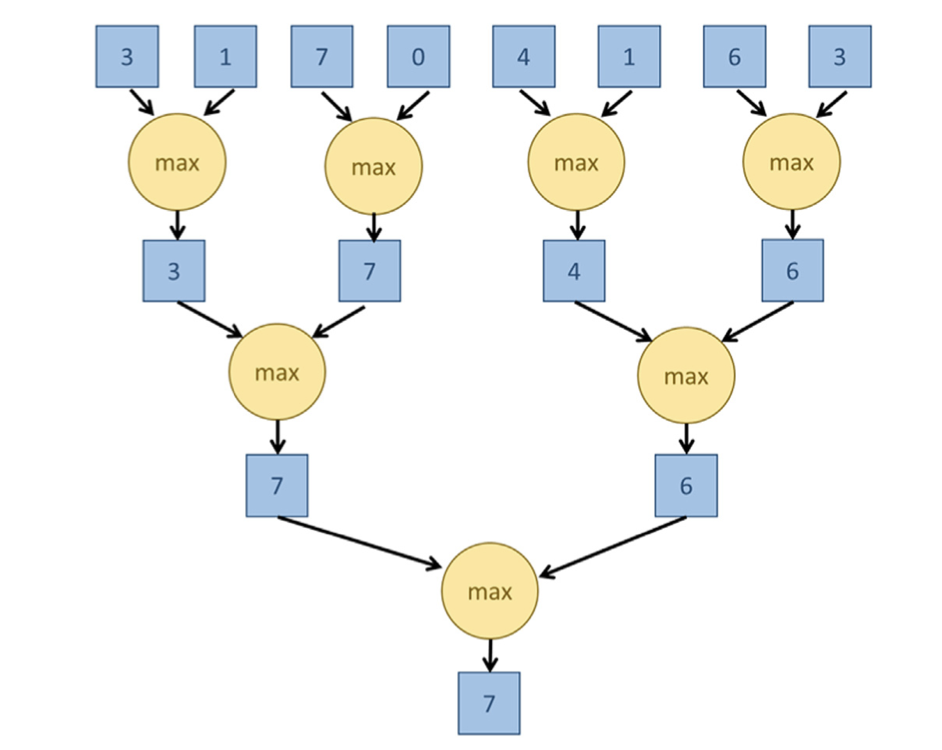
\includegraphics[width=0.9\textwidth]{figs/F10.3.png}
	\caption{\textit{并行最大归约树。}}
\end{figure}

并行归约算法已在文献中得到广泛研究。 并行归约的基本概念如图 10.3 所示,
其中时间在垂直方向上向下推进,线程在每个时间步中并行执行的活动在水平方向上显示。

在第一轮(时间步)期间,对四对原始元素并行执行四个最大操作。 这四个操作产生部分归约结果:来自四对原始元素的四个较大值。 
在第二个时间步中,对两对部分归约结果并行执行两个最大操作,并产生两个更接近最终归约结果的部分结果。 
这两个部分结果是原始输入中前四个元素的最大值和后四个元素的最大值。 
在第三个也是最后一个时间步长期间,执行一个 max 运算以生成最终结果,即原始输入的最大值 7。

请注意,执行操作的顺序将从顺序归约算法更改为并行归约算法。 
例如,对于图 10.3 顶部的输入,
像图 10.2 中那样的连续最大归约将首先通过将 acc 中的身份值 (2N) 与输入值 3 进行比较并用获胜者更新 acc 来开始, 即 3。
然后,它将比较 acc (3) 的值与输入值 1,并用获胜者(即 3)更新 acc。随后将 acc (3) 的值与输入值 7 进行比较, 
用获胜者更新 acc,即 7。然而,在图 10.3 的并行归约中,输入值 7 首先与输入值 0 进行比较,
然后再与 3 和 1 中的最大值进行比较。

正如我们所看到的,并行归约假设将运算符应用于输入值的顺序并不重要。 
在最大归约中,无论将运算符应用于输入值的顺序如何,结果都将是相同的。 如果运算符是结合的,则该属性在数学上得到保证。 
运算符 $\Theta$ 是结合的,如果 $(a-b) \Theta c=a \Theta(b \Theta c)$。 
例如,整数加法是结合的 $((1+2)+3=1+(2+3)=6)$,而整数减法是不结合的 $((1-2)-3 \neq 1-(2-3))$。
即 ,如果一个运算符具有结合性,则可以在涉及该运算符的表达式的任意位置插入括号,结果都相同。
利用这种等价关系,可以将运算符应用的任何顺序转换为任何其他顺序,
同时保持等价性 严格来说,浮点加法不具有关联性,因为引入括号的不同方式可能会导致舍入结果。
但是,如果浮点运算结果彼此之间的差异在可容忍的范围内,大多数应用程序都会接受相同的浮点运算结果。 
这样的定义使得开发人员和编译器编写者可以将浮点加法视为结合运算符,有兴趣的读者可以参考附录A了解详细处理。

从图 10.2 中的顺序归约到图 10.3 中的归约树的转换要求运算符具有结合性。 我们可以将归约视为一个操作列表。 
图 10.2 和图 10.3 之间的排序差异只是在同一列表的不同位置插入括号。 对于图 10.2,括号内为:
$$
((((((3)\max 1) \max 7) \max 0) \max 4) \max 1) \max 6) \max 3
$$

而图 10.3 的括号是:
$$
((3 \max 1) \max (7 \max 0)) \max ((4 \max 1) \max (6 \max 3))
$$

我们将在 10.4 节中应用优化,它不仅重新排列应用运算符的顺序,而且还重新排列操作数的顺序。 
为了重新排列操作数的顺序,这种优化还要求运算符是可交换的。 如果 $a \Theta b=b \Theta a$,则运算符是可交换的。 
也就是说,表达式中操作数的位置可以重新排列,结果是相同的。 
请注意,最大运算符也是可交换的,就像许多其他运算符(例如最小值、总和和乘积)一样。 
显然,并非所有运算符都是可交换的。 例如,加法是可交换的 ($1+2 = 2+1$),而整数减法则不可交换 ($1 - 2 \neq 2 - 1$)。

图 10.3 中的并行归约模式被称为归约树,因为它看起来像一棵树,其叶子是原始输入元素,其根是最终结果。 
不要将术语归约树与树数据结构混淆,在树数据结构中,节点要么显式地与指针链接,要么隐式地与分配的位置链接。 
在归约树中,边是概念性的,反映从一个时间步骤中执行的操作到下一时间步骤中执行的操作的信息流。

并行操作在产生最终结果所需的时间步数方面比顺序代码有了显着的改进。 
在图 10.3 的示例中,顺序代码中的 for 循环迭代八次,或采取八个时间步长,以访问所有输入元素并产生最终结果。 
另一方面,对于图 10.3 中的并行操作,并行归约树方法仅需要三个时间步骤:第一个时间步骤期间有四个最大操作,
第二个时间步骤期间有两个,第三个时间步骤期间有一个。 就时间步数而言,减少了 5/8 = 62.5\%,或者加速了 8/3 = 2.67。 
当然,并行方法是有代价的:必须有足够的硬件比较器才能在同一时间步长中执行最多四个操作。 
对于 N 个输入值,归约树在第一轮执行 $\frac{1}{2}N$ 次操作,在第二轮执行 $\frac{1}{4}N$ 次操作,依此类推。 
因此,执行的操作总数由几何级数 $\frac{1}{2} \mathrm{~N}+ \frac{1}{4} \mathrm{~N}+ \frac{1}{8} \mathrm{~N}+\ldots \frac{1}{N} \mathrm{N}=\mathrm{N}-1$ 定义,这与顺序算法类似。

就时间步长而言,归约树需要 $log_2 N$ 个步骤来完成 N 个输入值的归约过程。 
因此,假设有足够的执行资源,只需十步即可减少 $N = 1024$ 个输入值。 
第一步,我们需要 $1/2 N = 512$ 个执行资源! 请注意,随着时间步长的进展,所需的资源数量会迅速减少。 
在最后一个时间步骤中,我们只需要一个执行资源。 每个时间步的并行级别与所需的执行单元数量相同。 
计算所有时间步长的平均并行度很有趣。 平均并行度是执行的操作总数除以时间步数,即 $(N - 1)/log_2 N$。
对于 $N = 1024$,十个时间步的平均并行度为 102.3,而峰值并行度 是 512(在第一个时间步骤期间)。 
跨时间步长的并行级别和资源消耗的这种变化使得归约树成为并行计算系统中具有挑战性的并行模式。

\begin{figure}[H]
	\centering
	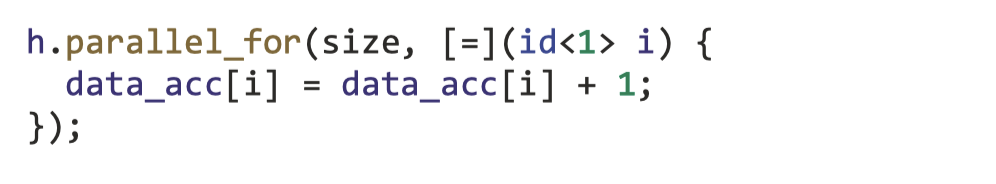
\includegraphics[width=0.9\textwidth]{figs/F10.5.png}
	\caption{\textit{并行求和归约树。}}
\end{figure}

图 10.5 显示了八个输入值的求和归约树示例。 
到目前为止,我们介绍的有关最大归约树的时间步数和资源消耗的所有内容也适用于求和归约树。 
使用最多四个加法器需要 $log_2 8 = 3$ 个时间步才能完成归约。 我们将使用这个例子来说明求和核的设计。

\begin{remark}[体育和比赛并行约化]
早在计算出现之前,并行归约就已经应用于体育和竞赛中。 图10.4显示了2010年南非世界杯四分之一决赛、半决赛和决赛的赛程表。 
应该清楚的是,这只是一个重新排列的归约树。 世界杯的淘汰过程是一种最大归约,即最大算子返回“击败”对方球队的球队。 
锦标赛“归约”是多轮进行的。 各队被分成两人一组。 在第一轮比赛中,所有双人组并行比赛。 
第一轮的获胜者晋级第二轮,第二轮的获胜者晋级第三轮,以此类推。 
八支球队参加比赛,第一轮(图 10.4 中的四分之一决赛)产生四名获胜者,第二轮(图 10.4 中的半决赛)产生两名获胜者,
第三轮(图 10.4 中的决赛)产生一名最终获胜者(冠军)。 图 10.4)。 每轮都是归约过程的一个时间步。

\begin{figure}[H]
	\centering
	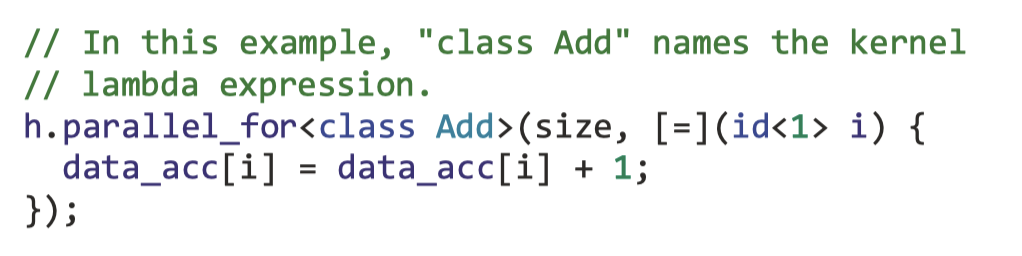
\includegraphics[width=0.9\textwidth]{figs/F10.4.png}
	\caption{\textit{2010年世界杯决赛作为一棵还原树。}}
\end{figure}

应该很容易看出,即使有1024支球队,也只需要10轮就可以确定最终的获胜者。 
诀窍是要有足够的资源来并行举办第一轮的512场比赛、第二轮的256场比赛、第三轮的128场比赛,以此类推。 
在资源充足的情况下,即使是6万支队伍,也只需16轮就能决出最后的胜者。 
有趣的是,虽然归约树可以大大加快归约过程,但它们也消耗相当多的资源。 
以世界杯为例,一场比赛需要一个大型足球场、官员和工作人员以及酒店和餐馆来容纳大量观众。 
图 10.4 中的四场四分之一决赛在三个城市(纳尔逊·曼德拉湾/伊丽莎白港、开普敦和约翰内斯堡)进行,
这三个城市共同提供了足够的资源来举办四场比赛。 请注意,约翰内斯堡的两场比赛是在不同的两天进行的。 
因此,两个游戏之间共享资源使得归约过程需要更多时间。 我们将在计算归约树中看到类似的权衡。
\end{remark}

\subsection{简单的归约核函数}
我们现在准备开发一个简单的内核来执行图 10.5 所示的并行求和归约树。 
由于归约树需要跨所有线程协作,而这在整个网格中是不可能的,因此我们将首先实现一个在单个块内执行求和归约树的内核。 
也就是说,对于 N 个元素的输入数组,我们将调用这个简单内核,并启动一个包含 $\frac{1}{2}$N 个线程块的网格。 
由于一个块最多可以有 1024 个线程,因此我们最多可以处理 2048 个输入元素。 我们将在第 10.8 节中消除此限制。 
在第一个时间步中,所有 $\frac{1}{2}$N 个线程都会参与,每个线程将两个元素相加以产生 $\frac{1}{2}$N 个部分和。 
在下一个时间步中,一半线程将退出,只有 $\frac{1}{4}$N 个线程将继续参与生成 $\frac{1}{2}$N 部分和。 
此过程将持续到最后一个时间步,其中仅保留一个线程并生成总和。

\begin{figure}[H]
	\centering
	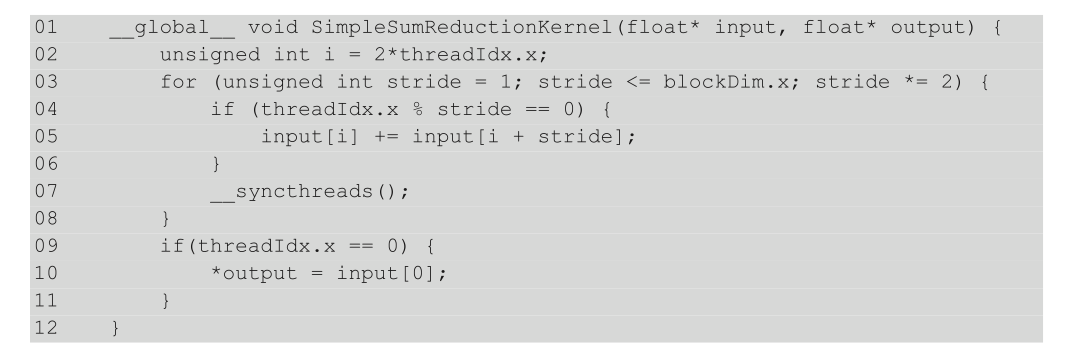
\includegraphics[width=0.9\textwidth]{figs/F10.6.png}
	\caption{\textit{一个简单的求和归约内核。}}
\end{figure}

\begin{figure}[H]
	\centering
	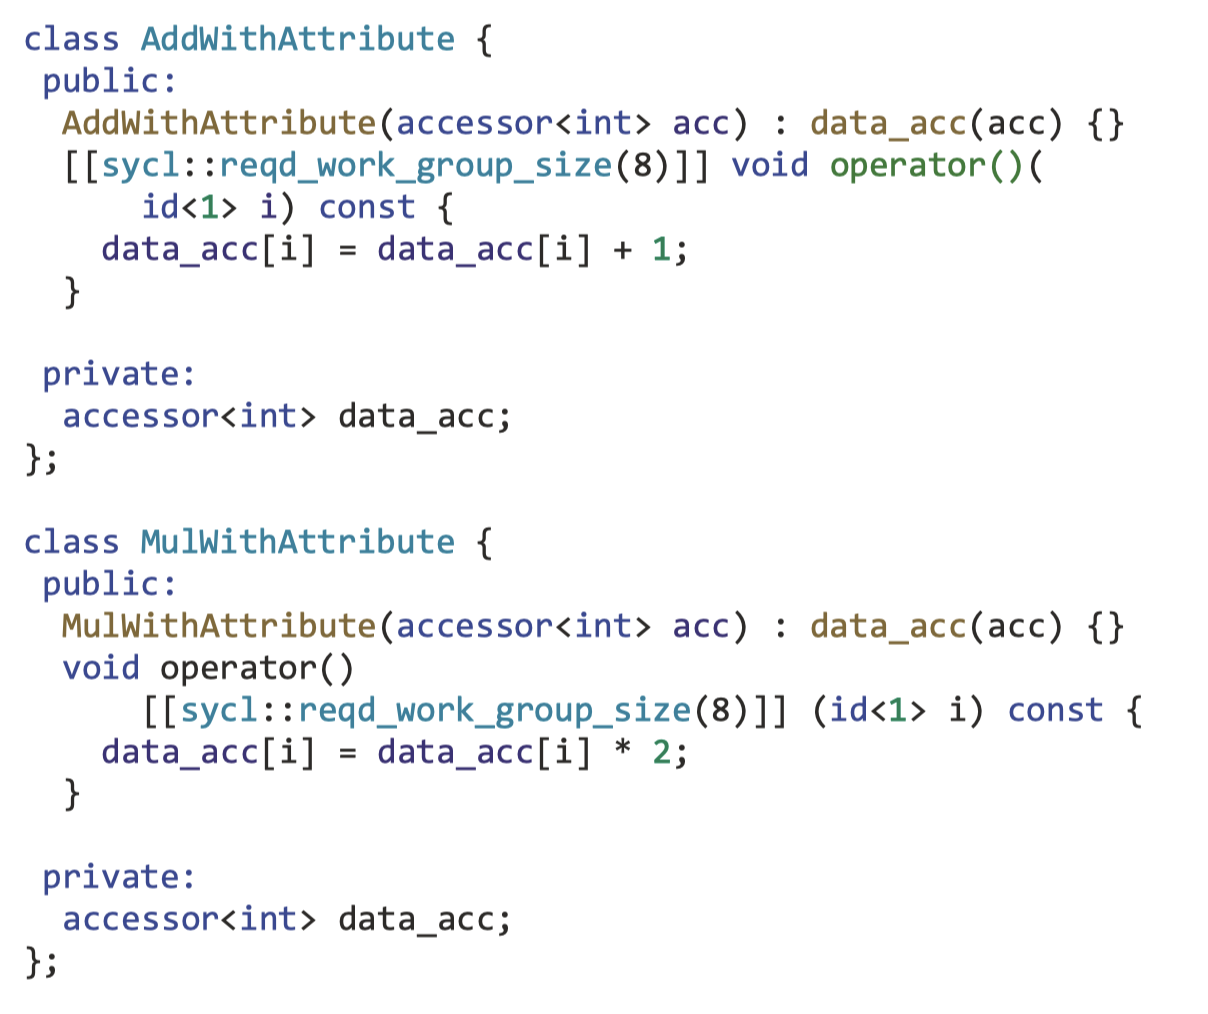
\includegraphics[width=0.9\textwidth]{figs/F10.7.png}
	\caption{\textit{图 10.6 中 SimpleSumReudctionKernel 的线程(“所有者”)到输入数组位置的分配以及随着时间的推移执行进度。 时间从上到下进行,每一级对应于 for 循环的一次迭代。}}
\end{figure}

图 10.6 显示了简单求和核函数的代码,图 10.7 说明了由该代码实现的归约树的执行。 
请注意,在图 10.7 中,时间是从上到下进行的。 
我们假设输入数组位于全局内存中,并且在调用内核函数时将指向该数组的指针作为参数传递。 
每个线程都被分配到一个数据位置,即 2 * threadIdx.x(第 02 行)。 
也就是说,线程被分配到输入数组中的偶数位置:线程 0 分配到 input[0],线程 1 分配到 input[2],
线程 2 分配到 input[4],依此类推,如顶行所示 图10.7。 
每个线程都将是其所分配到的位置的“所有者”,并且是写入该位置的唯一线程。 
内核的设计遵循“所有者计算”方法,其中每个数据位置都由唯一的线程拥有,并且只能由该所有者线程更新。

图 10.7 的顶行显示了线程对输入数组位置的分配,随后的每一行显示了每个时间步对输入数组位置的写入,
即图 10.7 中 for 循环的迭代 . 10.6(第 03 行)。 
内核在 for 循环的每次迭代中覆盖的位置被标记为图 10.7 中输入数组的填充位置。 
例如,在第一次迭代结束时,具有偶数索引的位置将被输入数组中原始元素对(0+1、2+3、4+5 等)的部分和覆盖。 
在第二次迭代结束时,索引为 4 倍数的位置将被输入数组中四个相邻原始元素(0+3、4+7 等)的部分和覆盖。

在图 10.6 中,线程使用跨步变量来获取适当的部分和以累积到其所有者位置。 stride 变量初始化为 1(第 03 行)。 
stride 变量的值在每次迭代中加倍,因此 stride 变量值将为 1、2、4、8 等,直到它大于 blockIdx.x(块中的线程总数)。 
如图 10.7 所示,迭代中的每个活动线程使用步幅变量将步幅距离的输入数组元素添加到其拥有的位置。 
例如,在迭代 1 中,线程 0 使用步幅值 1 将 input[1] 添加到其拥有的位置 input[0] 中。 
这会将 input[0] 更新为 input[0] 和 input[1] 的第一对原始值的部分和。 
在第二次迭代中,线程 0 使用步幅值 2 将 input[2] 添加到 input[0]。 
此时,input[2]包含input[2]和input[3]原始值之和,input[0]包含input[0]和input[1]原始值之和。 
因此,在第二次迭代之后,input[0] 包含输入数组前四个元素的原始值之和。 
最后一次迭代后,input[0] 包含输入数组所有原始元素的总和,从而得到总和归约的结果。 
该值由线程 0 写入作为最终输出(第 10 行)。

我们现在转向图 10.6 中的 if 语句(第 04 行)。 if 语句的条件设置为在每次迭代中选择活动线程。 
如图10.7所示,在迭代 n 期间,线程索引(threadIdx.x)值为 $2^n$ 的倍数的线程将执行加法。 
条件为threadIdx.x \% stride == 0,测试线程索引值是否为stride变量值的倍数。 
回想一下,步幅的值为 $1, 2, 4, 8, \ldots$ 。 通过迭代,或 $2^n$ 表示迭代 n。 
因此,该条件确实测试线程索引值是否是 $2^n$ 的倍数。 回想一下,所有线程都执行相同的内核代码。 
线程索引值满足if条件的线程是执行加法语句的活动线程(第05行)。 线程索引值不满足条件的线程是跳过加法语句的非活动线程。 
随着迭代的进行,保持活动状态的线程越来越少。 在最后一次迭代中,只有线程 0 保持活动状态并生成求和结果。

for 循环中的 \_\_syncthreads() 语句(图 10.6 的第 07 行)确保在允许任何一个线程开始迭代之前,
迭代计算出的所有部分和都已写入输入数组中的目标位置。 下一次迭代。 
这样,进入迭代的所有线程都将能够正确使用上一次迭代中生成的部分和。 
例如,在第一次迭代之后,偶数元素将被成对部分和替换。 
\_\_syncthreads() 语句确保第一次迭代中的所有这些部分和确实已写入输入数组的偶数位置,并准备好由第二次迭代中的活动线程使用。

\subsection{最小化控制分支}
图 10.6 中的内核代码实现了图 10.7 中的并行归约树并产生了预期的求和归约结果。 
不幸的是,它在每次迭代中对活动和非活动线程的管理导致了高度的控制分支。 
例如,如图10.7所示,只有那些threadIdx.x值为偶数的线程才会在第二次迭代期间执行加法语句。 
正如我们在第 4 章“计算架构和调度”中所解释的,控制发散会显着降低执行资源利用效率,或用于生成有用结果的资源百分比。 
在这个例子中,一个warp中的所有32个线程都消耗执行资源,但只有一半是活动的,浪费了一半的执行资源。 
由于分支而造成的执行资源浪费随着时间的推移而增加。 
在第三次迭代期间,warp 中只有四分之一的线程处于活动状态,浪费了四分之三的执行资源。 
在迭代 5 期间,warp 中的 32 个线程中只有 1 个处于活动状态,浪费了 32 / 31 的执行资源。

如果输入数组的大小大于 32,则第五次迭代后整个warp将变为非活动状态。 
例如,对于 256 的输入大小,将启动 128 个线程或四个warp。 
所有四个warp都将具有相同的发散模式,正如我们在上一段中针对迭代 1 到 5 所解释的那样。
在第六次迭代期间,warp 1 和warp 3 将完全不活动,因此不会表现出控制发散。 
另一方面,warp 0 和 warp 2 将只有一个活动线程,表现出控制分支并浪费 31 / 32 的执行资源。 
在第七次迭代期间,只有 warp 0 处于活动状态,表现出控制发散并浪费了 31 / 32 的执行资源。

一般来说,大小为 N 的输入数组的执行资源利用效率可以计算为活动线程总数与消耗的执行资源总数之间的比率。 
消耗的执行资源总数与所有迭代中的活动warp总数成正比,因为每个活动warp,无论其活动线程有多少,都会消耗全部执行资源。 
这个数字可以计算如下:
$$
\left(\mathrm{N} / 64 * 5+\mathrm{N} / 64 * \frac{1}{2} +\mathrm{N} / 64*\frac{1}{4} +\ldots+1\right) * 32
$$

这里,N/64 是启动的 warp 总数,因为将启动 N/2 个线程,每 32 个线程形成一个 warp。 
N/64 项乘以 5,因为所有启动的warp在五次迭代中都处于活动状态。 第五次迭代之后,每次连续迭代中的warp数量减少一半。 
括号中的表达式给出了所有迭代中活动warp的总数。 
第二项反映每个活动 warp 都会消耗所有 32 个线程的全部执行资源,无论这些 warp 中的活动线程数量如何。 
对于输入数组大小为 256 的情况,消耗的执行资源为 $(4 * 5+2+1) × 32 = 736$。

活动线程提交的执行结果数是所有迭代中活动线程的总数:
$$
\mathrm{N} / 64 * (32+16+8+4+2+1)+\mathrm{N} / 64*\frac{1}{2} * 1+\mathrm{N} / 64* \frac{1}{4}* 1+\ldots+1
$$

括号中的项给出了所有 N/64 warp 的前五次迭代中的活动线程。 
从第六次迭代开始,每次迭代中活动warp的数量减少一半,并且每个活动warp中只有一个活动线程。 
对于大小为 256 的输入数组,提交结果的总数为 $4*(32+16+8+4+2+1)+2+1 = 255$。
这个结果应该很直观,因为 减少 256 个值所需的是 255。

将前两个结果放在一起,我们发现输入数组大小为256时的执行资源利用效率为 $255/736 = 0.35$。 
该比率表明并行执行资源没有充分发挥加速计算的潜力。 平均而言,仅约 35\% 的消耗资源对总量减少结果做出了贡献。 
也就是说,我们只使用了大约 35\% 的硬件潜力来加速计算。

基于此分析,我们发现跨warp和时间推移存在广泛的控制分支。 
正如读者可能想知道的那样,可能有更好的方法将线程分配到输入数组位置,以减少控制发散并提高资源利用效率。 
图 10.7 所示分配的问题在于,部分和位置彼此之间的距离越来越远,
因此,随着时间的推移,拥有这些位置的活动线程彼此之间的距离也越来越远。 活动线程之间距离的增加导致控制发散程度的增加。

\begin{figure}[H]
	\centering
	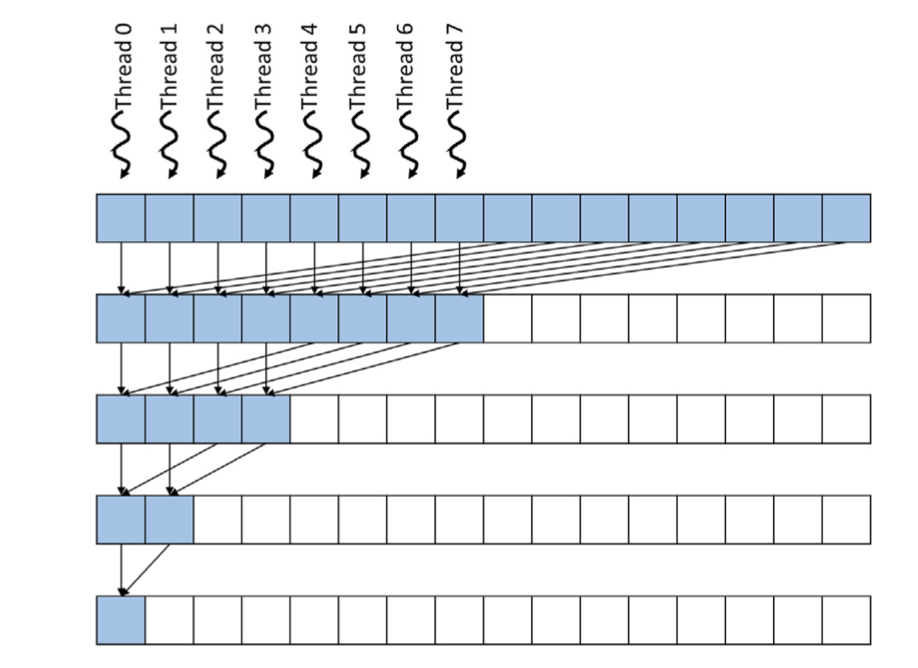
\includegraphics[width=0.9\textwidth]{figs/F10.8.png}
	\caption{\textit{更好地将线程分配到输入数组位置以减少控制分歧。}}
\end{figure}

确实有更好的分配策略可以显着减少控制发散。 我们的想法是,我们应该安排线程及其所属位置,
以便随着时间的推移它们可以保持彼此靠近。 也就是说,我们希望步幅值随着时间的推移而减小,而不是增加。 
对于 16 个元素的输入数组,修改后的分配策略如图 10.8 所示。 在这里,我们将线程分配到前半部分位置。 
在第一次迭代期间,每个线程到达输入数组的一半,并将输入元素添加到其所有者位置。 
在我们的示例中,线程 0 将 input[8] 添加到其拥有的位置 input[0],线程 1 将 input[9] 添加到其拥有的位置 input[1],
依此类推。 在每次后续迭代期间,一半的活动线程会消失,所有剩余的活动线程都会添加一个输入元素,
该元素的位置是距其所有者位置的活动线程的数量。 
在我们的示例中,在第三次迭代期间,有两个剩余的活动线程:线程 0 将 input[2] 添加到其拥有的位置 input [0],
线程 1 将 input[3] 添加到其拥有的位置 input[1]。 
请注意,如果我们将图 10.8 与图 10.7 的操作和操作数顺序进行比较,就会发现列表中的操作数实际上进行了重新排序,
而不仅仅是以不同方式插入括号。 为了使这种重新排序的结果始终保持相同,该操作必须是可交换的以及结合的。

\begin{figure}[H]
	\centering
	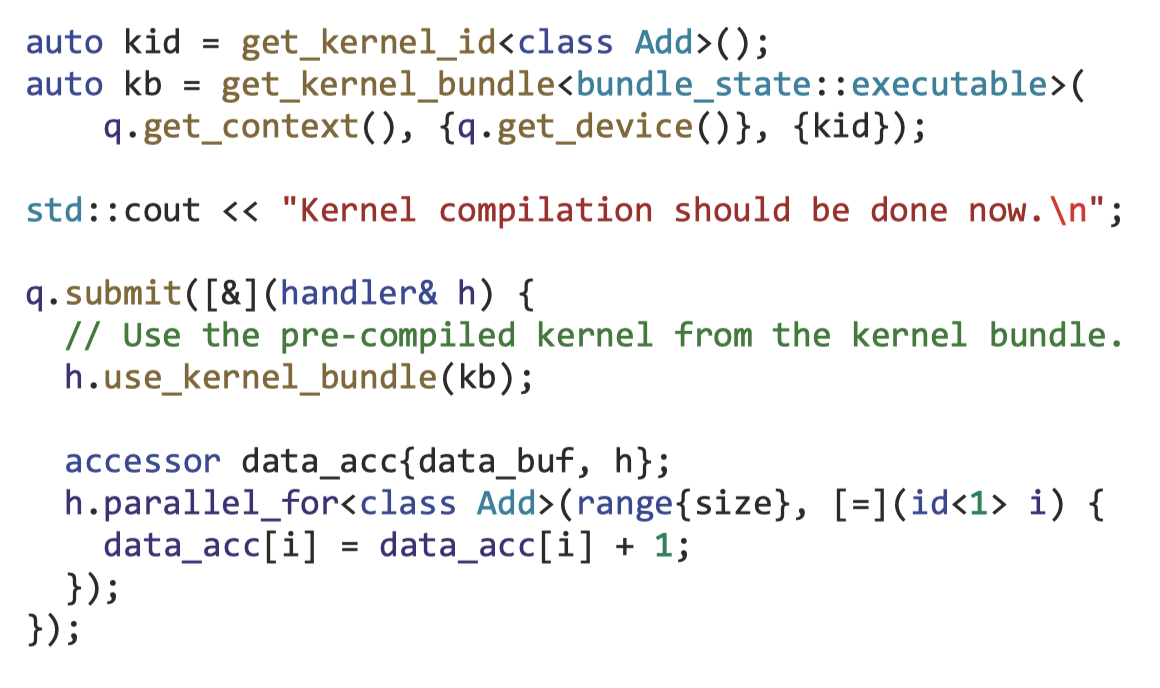
\includegraphics[width=0.9\textwidth]{figs/F10.9.png}
	\caption{\textit{控制发散较小、执行资源利用效率提高的内核。}}
\end{figure}

图 10.9 显示了对图 10.6 中的简单内核进行了一些微妙但关键的更改的内核。 
所有者位置变量 i 设置为 threadIdx.x,而不是 2 * threadIdx.x(第 02 行)。 
因此,所有线程的所有者位置现在彼此相邻,如图 10.8 所示。 
步长值被初始化为 blockDim.x 并减少一半,直到达到 1(第 03 行)。 
在每次迭代中,只有索引小于步幅值的线程保持活动状态(第 04 行)。 因此,所有活动线程都有连续的线程索引,如图 10.8 所示。 
它不是在第一轮中添加相邻元素,而是添加彼此相距半个段的元素,并且段大小始终是剩余活动线程数的两倍。 
在第一轮中添加的所有对都彼此远离 blockDim.x。 第一次迭代后,所有成对和都存储在输入数组的前半部分中,如图 10.8 所示。 
该循环在进入下一次迭代之前将步幅除以 2。 因此,对于第二次迭代,步幅变量值是 blockDim.x 值的一半。 
也就是说,剩余的活动线程在第二次迭代期间添加彼此相距四分之一节的元素。

图 10.9 中的内核在循环中仍然有一个 if 语句(第 04 行)。 
每次迭代中执行加法运算(第 06 行)的线程数与图 10.6 中的相同。 
那么为什么两个内核之间的控制分支会存在差异呢? 答案在于执行加法操作的线程相对于不执行加法操作的线程的位置。 
让我们考虑一个包含 256 个元素的输入数组的示例。 在第一次迭代期间,所有线程都处于活动状态,因此不存在控制分支。 
在第二次迭代期间,线程 0 到 63 执行 add 语句(活动),而线程 64 到 127 则不执行(非活动)。 
在第二次迭代期间,两两求和存储在元素 0 到 63 中。 
由于 warp 由具有连续 threadIdx.x 值的 32 个线程组成,因此 warp 0 到 warp 1 中的所有线程都执行 add 语句,
而 warp 2 到 warp 3 中的所有线程都变为非活动状态。 
由于每个 warp 中的所有线程都采用相同的执行路径,因此不存在控制分支!

然而,图10.9中的内核并没有完全消除由if语句引起的分支。 
读者应该验证一下,对于 256 个元素的示例,从第四次迭代开始,执行加法运算的线程数将降至 32 以下。
也就是说,最后五次迭代将只有 16, 8, 4, 2, 和 1 个线程执行加法。 这意味着内核执行在这些迭代中仍然会存在分支。 
然而,具有分支的循环的迭代次数从十次减少到五次。 我们可以计算消耗的执行资源总数如下:
$$
\left(\mathrm{N} / 64 * 1+\mathrm{N} / 64 * \frac{1}{2}+\ldots+1+5* 1\right)* 32
$$

括号中的部分反映了这样一个事实:在每次后续迭代中,一半的warp变得完全不活动并且不再消耗执行资源。 
这个系列一直持续到只有一个完整的活动线程warp为止。 
最后一项 (5 × 1) 反映了这样一个事实:对于最后五次迭代,只有一个活动warp,并且其所有 32 个线程都消耗执行资源,
即使只有一小部分线程处于活动状态。 因此,括号中的总和给出了所有迭代中的 warp 执行总数,乘以 32 后得出消耗的执行资源总量。

对于我们的 256 个元素的示例,消耗的执行资源为 $(4+2+1+5 × 1) × 32 = 384$,
几乎是图 10.6 中内核消耗的资源 736 的一半。 
由于每次迭代中的活动线程数从图 10.7 到图 10.8 没有变化,
因此图 10.9 中新内核的效率为 $255/384 = 66\%$,几乎是图 10.6 中内核效率的两倍。 
另请注意,由于线程束被安排在执行资源有限的流式多处理器中轮流执行,因此总执行时间也将随着资源消耗的减少而提高。

图 10.6 和图 10.9 中的内核之间的差异很小,但会对性能产生重大影响。 
它需要对设备的单指令、多数据硬件上的线程执行有清晰了解的人员才能自信地进行此类调整。

\subsection{最小化内存分支}
图 10.6 中的简单内核还有另一个性能问题:内存分支。 
正如我们在第 5 章“内存架构和数据局部性”中所解释的,在每个 warp 内实现内存合并非常重要。 
也就是说,warp 中的相邻线程在访问全局内存时应该访问相邻位置。 
不幸的是,在图 10.7 中,相邻线程不访问相邻位置。 在每次迭代中,每个线程执行两次全局内存读取和一次全局内存写入。 
第一次读取是从其拥有的位置开始的,第二次读取是从与其拥有的位置相距一定距离的位置开始的,而写入则是从其拥有的位置开始的。 
由于相邻线程拥有的位置不是相邻位置,因此相邻线程进行的访问将不会完全合并。 
在每次迭代期间,由warp共同访问的内存位置彼此之间存在跨距距离。

例如,如图 10.7 所示,当 warp 中的所有线程在第一次迭代期间执行其第一次读取时,位置彼此相距两个元素。 
结果会触发两次全局内存请求,返回的数据有一半不会被线程使用。 第二次读取和写入时会发生相同的行为。 
在第二次迭代期间,所有其他线程都会退出,并且warp共同访问的位置彼此相距四个元素。 
再次执行两次全局内存请求,返回的数据中只有四分之一会被线程使用。 
这将持续下去,直到每个warp只有一个活动线程保持活动状态。 
仅当 warp 中存在 1 个活动线程时,warp 才会执行一次全局内存请求。 因此全局内存请求总数如下:
$$
\left(\mathrm{N} / 64* 5* 2+\mathrm{N} / 64* 1+\mathrm{N} / 64*\frac{1}{2}+\mathrm{N} / 64*\frac{1}{4}+\ldots+1\right)* 3
$$

第一项 (N/64 * 5 * 2) 对应于前五次迭代,其中所有 N/64 warp 都有两个或更多活动线程,
因此每个 warp 执行两个全局内存请求。 其余项说明最终迭代,其中每个 warp 只有一个活动线程并执行一个全局内存请求,
并且在每次后续迭代中都会有一半的 warp 退出。 乘以 3 表示每次迭代期间每个活动线程进行两次读取和一次写入。 
在 256 个元素的示例中,全局内存请求的内核执行的总数是 $(4 * 5 * 2+4+2+1) * 3 = 141$。

对于图 10.9 中的内核,每个 warp 中的相邻线程总是访问全局内存中的相邻位置,因此访问总是合并的。 
因此,每个 warp 在任何读取或写入时仅触发一个全局内存请求。 
随着迭代的进行,整个 warp 都会消失,因此这些非活动 warp 中的任何线程都不会执行全局内存访问。 
每次迭代中都会有一半的warp消失,直到最后五次迭代只剩下一个warp。 因此内核执行的全局内存请求总数如下:
$$
\left(\left(\mathrm{N} / 64+\mathrm{N} / 64*\frac{1}{2}+\mathrm{N} / 64*\frac{1}{4}+\ldots+1\right)+5\right)* 3
$$

对于 256 个元素的示例,执行的全局内存请求总数为 $((4+2+1)+5) * 3 = 36$。
改进后的内核导致全局内存请求减少了 $141/36 = 3.9\times$。 
由于 DRAM 带宽是有限的资源,因此图 10.6 中的简单内核的执行时间可能会明显更长。

对于 2048 个元素的示例,图 10.6 中内核执行的全局内存请求总数为 $(32 * 5 * 2+32+16+8+4+2+1) * 3 = 1149$,
而 图 10.9 中内核执行的全局内存请求的数量为 $(32+16+8+4+2+1+5) * 3 = 204$。比率为 5.6,
甚至比 256 元素示例中的比率还要高 。 
这是因为图 10.6 中内核的低效执行模式,其中在执行的最初五次迭代期间有更多的活动 warp,
并且每个活动 warp 触发的全局内存请求数量是图 10.9 中收敛内核的两倍。

总之,收敛内核在使用执行资源和 DRAM 带宽方面提供了更高的效率。 其优势来自于减少的控制发散和改进的内存合并。

\subsection{极小化全局内存访问}
图10.9中的收敛内核可以通过使用共享内存进一步改进。 
请注意,在每次迭代中,线程将其部分求和结果值写入全局内存,并且这些值将由相同线程和其他线程在下一次迭代中重新读取。 
由于共享内存比全局内存具有更短的延迟和更高的带宽,因此我们可以通过将部分求和结果保留在共享内存中来进一步提高执行速度。 
这个想法如图 10.10 所示。

\begin{figure}[H]
	\centering
	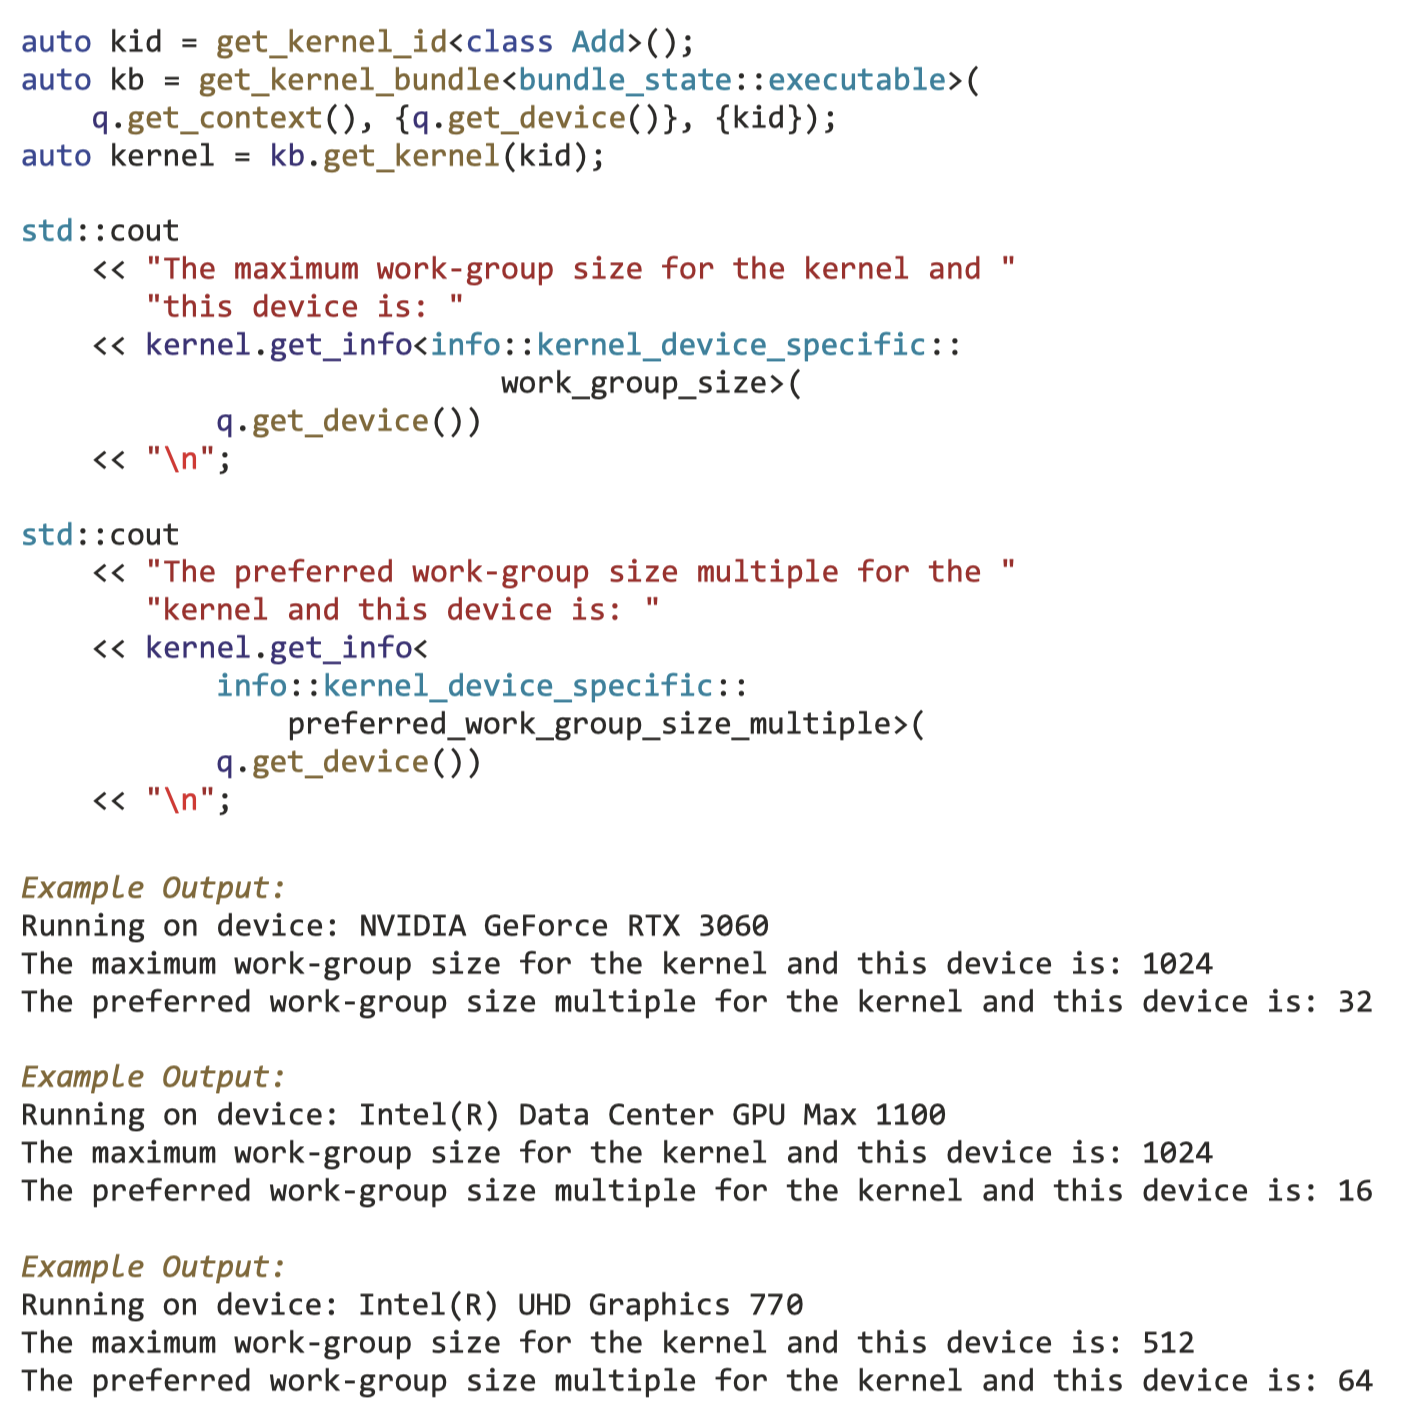
\includegraphics[width=0.9\textwidth]{figs/F10.10.png}
	\caption{\textit{使用共享内存来减少对全局内存的访问。}}
\end{figure}

\begin{figure}[H]
	\centering
	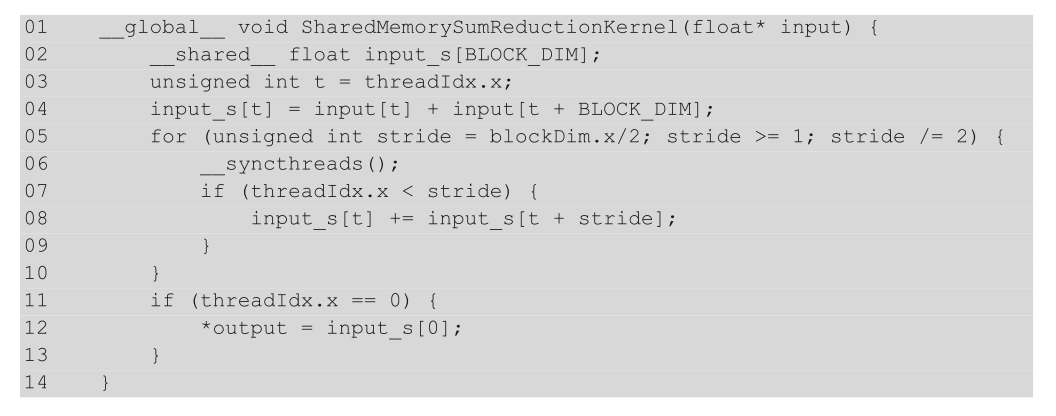
\includegraphics[width=0.9\textwidth]{figs/F10.11.png}
	\caption{\textit{使用共享内存来减少全局内存访问的内核。}}
\end{figure}

使用共享内存的策略在图10.11所示的内核中实现。 
这个想法是使用每个线程加载并添加两个原始元素,然后将部分和写入共享内存(第 04 行)。 
由于在访问循环外部的全局内存位置时已经完成了第一次迭代,
因此 for 循环从 blockDim.x/2 (第 04 行)而不是 blockDim.x 开始。 
\_\_syncthreads() 被移动到循环的开头,以确保我们在共享内存访问和循环的第一次迭代之间进行同步。 
线程通过读取和写入共享内存来继续剩余的迭代(第 08 行)。 
最后,在内核末尾,线程 0 将总和写入输出,保持与之前内核相同的行为(第 11-13 行)。

使用图 10.11 中的内核,全局内存访问的次数减少到初始加载输入数组的原始内容和最终写入 input[0]。 
因此,对于 N 元素归约,全局内存访问的数量仅为 N+1。 另请注意,图 10.11(第 04 行)中的两个全局内存读取都是合并的。 
因此,通过合并,只会有 (N/32) +1 个全局内存请求。 
对于 256 个元素的示例,触发的全局内存请求总数将从图 10.9 中内核的 36 个减少到图 10.10 中共享内存内核的 $8+1 = 9$,
即 $4\times$ 的改进。 除了减少全局内存访问次数之外,使用共享内存的另一个好处是输入数组不会被修改。 
如果程序的另一部分中的某些其他计算需要数组的原始值,则此属性非常有用。

\subsection{任意输入长度的分层归约}
到目前为止,我们研究的所有内核都假设它们将通过一个线程块启动。 
这种假设的主要原因是 \_\_syncthreads() 用作所有活动线程之间的屏障同步。 
回想一下,\_\_syncthreads() 只能在同一块中的线程之间使用。 这将当前硬件上的并行级别限制为 1024 个线程。 
对于包含数百万甚至数十亿个元素的大型输入数组,我们可以通过启动更多线程来进一步加速归约过程。 
由于我们没有一个好的方法来在不同块中的线程之间执行屏障同步,因此我们需要允许不同块中的线程独立执行。

\begin{figure}[H]
	\centering
	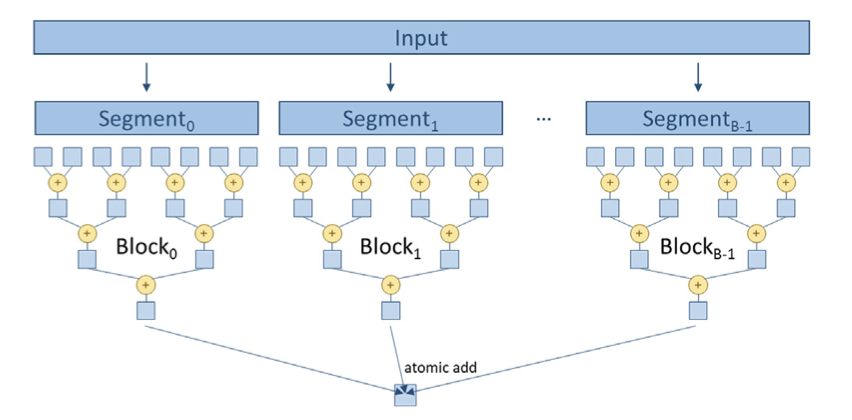
\includegraphics[width=0.9\textwidth]{figs/F10.12.png}
	\caption{\textit{使用原子操作进行分段多块缩减。}}
\end{figure}

\begin{figure}[H]
	\centering
	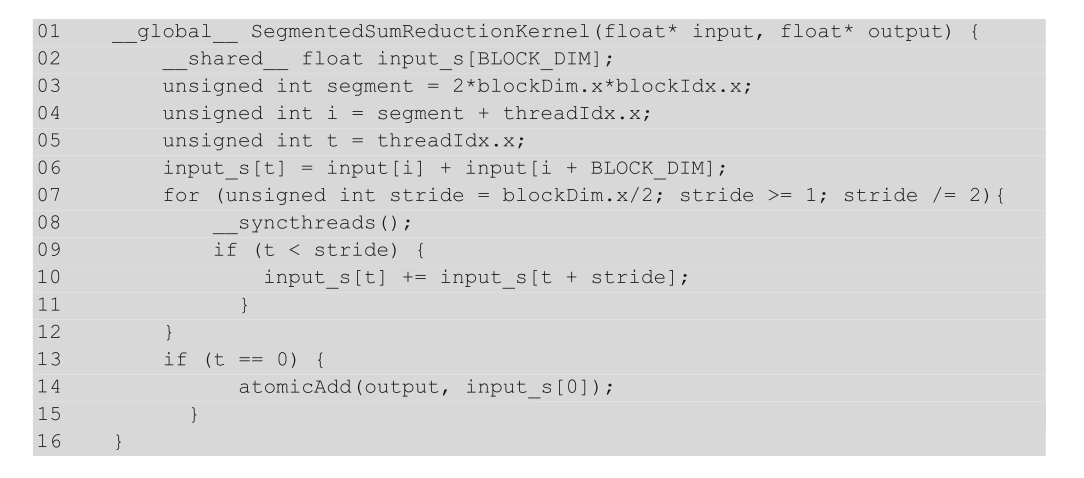
\includegraphics[width=0.9\textwidth]{figs/F10.13.png}
	\caption{\textit{使用原子操作的分段多块求和缩减内核。}}
\end{figure}

图 10.12 说明了使用原子操作进行分层、分段多块归约的概念,图 10.13 显示了相应的内核实现。 
这个想法是将输入数组划分为多个段,以便每个段对于一个块来说具有适当的大小。 
然后,所有块独立执行归约树,并使用原子添加操作将其结果累积到最终输出。

分区是通过根据线程的块索引为段变量分配不同的值来完成的(第 03 行)。 每个段的大小为 2 × blockDim.x。 
也就是说,每个块处理 2 × blockDim.x 元素。 
因此当我们将每个段的大小乘以块的 blockIdx.x,我们就得到了该块要处理的段的起始位置。 
例如,如果一个块中有 1024 个线程,则段大小将为 2 × 1024 5 2048。段的起始位置对于块 0 为 0,
对于块 1 为 2048 (2048 × 1),对于块 1 为 4096 (2048 × 2) ) 对于块 2,依此类推。

一旦我们知道每个块的起始位置,块中的所有线程就可以简单地处理分配的段,就好像它是整个输入数据一样。 
在块内,我们通过将 threadIdx.x 添加到线程所属块的段起始位置(第 04 行)来将拥有的位置分配给每个线程。 
局部变量 i 保存线程在全局输入数组中的拥有位置,而 t 保存线程在共享 input\_s 数组中的拥有位置。 
第 06 行适合在访问全局输入数组时使用 i 而不是 t。 图 10.11 中的 for 循环没有改变地使用。 
这是因为每个块在共享内存中都有自己的私有 input\_s,因此可以使用 t = threadIdx.x 访问它,就好像该段是整个输入一样。

一旦归约树 for 循环完成,该段的部分和就位于 input\_s[0] 中。 
图 10.13 第 16 行的 if 语句选择线程 0 将 input\_s[0] 中的值贡献给输出,如图 10.12 底部所示。 
这是通过原子添加完成的,如图 10.13 的第 14 行所示。 
一旦网格的所有块都完成执行,内核将返回,并且总和位于输出指向的内存位置中。

\subsection{线程粗化以减少开销}
到目前为止,我们使用的归约内核都试图通过使用尽可能多的线程来最大化并行性。 
也就是说,为了减少N个元素,启动N/2个线程。 如果线程块大小为 1024 个线程,则所得线程块数为 N/2048。 
然而,在执行资源有限的处理器中,硬件可能仅具有足够的资源来并行执行一部分线程块。 
在这种情况下,硬件将序列化多余的线程块,每当旧线程块完成时就执行新的线程块。

为了并行化归约,我们实际上付出了沉重的代价,将工作分配到多个线程块上。 
正如我们在前面几节中看到的,硬件利用率随着归约树的每个连续阶段而增加,因为更多的warp变得空闲,
并且最终的warp经历了更多的控制发散。 我们启动的每个线程块都会出现硬件未充分利用的阶段。 
如果线程块要真正并行运行,这是不可避免的代价。 但是,如果硬件要序列化这些线程块,我们最好自己以更有效的方式序列化它们。 
正如我们在第 6 章“性能注意事项”中讨论的那样,线程粒度粗化或简单来说线程粗化是一类优化,
它将某些工作序列化为更少的线程以减少并行化开销。 我们首先展示通过为每个线程块分配更多元素来应用线程粗化的并行归约的实现。 
然后,我们进一步详细说明此实现如何减少硬件利用率不足。

\begin{figure}[H]
	\centering
	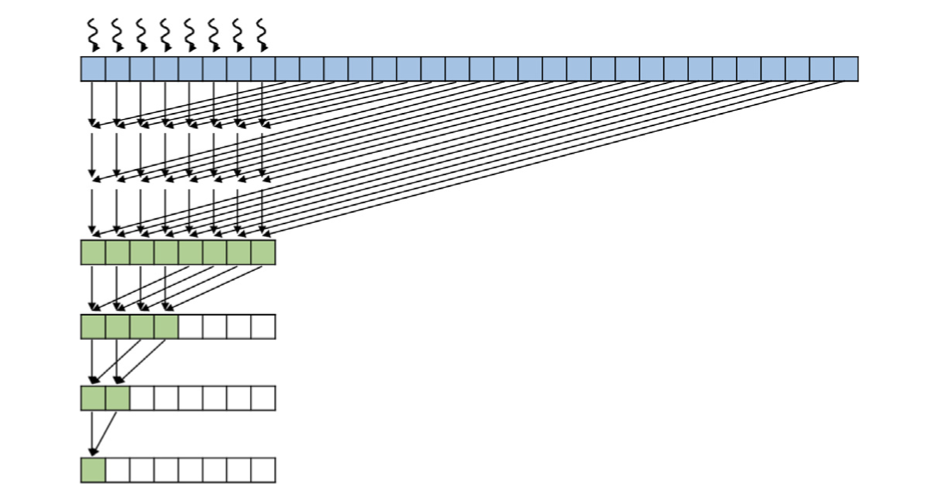
\includegraphics[width=0.9\textwidth]{figs/F10.14.png}
	\caption{\textit{归约中的线程粗化。}}
\end{figure}

图 10.14 说明了如何将 warp 粗化应用于图 10.10 中的示例。 在图 10.10 中,每个线程块接收 16 个元素,即每个线程两个元素。 
每个线程独立地添加它负责的两个元素; 然后线程协作执行归约树。 在图 10.14 中,我们将线程块粗化了 2 倍。
因此,每个线程块接收两倍数量的元素,即 32 个元素,即每个线程 4 个元素。 
在这种情况下,每个线程在协作执行归约树之前独立添加四个元素。 添加四个元素的三个步骤如图 10.14 中的前三行箭头所示。 
请注意,在这三个步骤中所有线程都处于活动状态。 
此外,由于线程独立地添加它们负责的四个元素,因此它们不需要同步,
并且它们不需要在添加所有四个元素之前将它们的部分和存储到共享内存。 执行归约树的其余步骤与图 10.10 中的相同。

\begin{figure}[H]
	\centering
	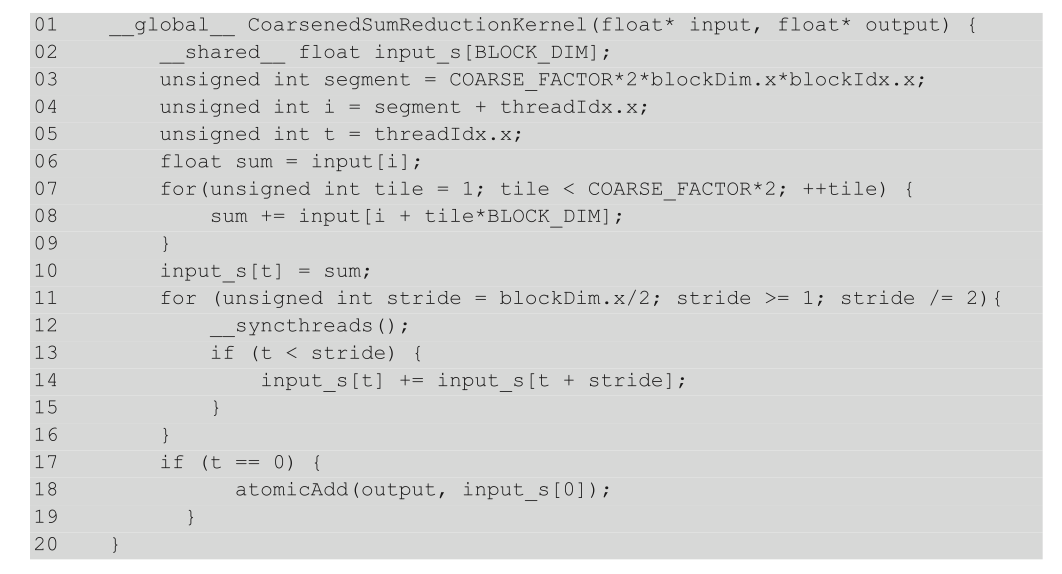
\includegraphics[width=0.9\textwidth]{figs/F10.15.png}
	\caption{\textit{带有线程粗化的求和归约内核。}}
\end{figure}

图 10.15 显示了通过多块分段内核的线程粗化实现归约的内核代码。 与图 10.13 相比,内核有两个主要区别。 
第一个区别是,当识别出块段的开头时,我们乘以 COARSE\_FACTOR 以反映块段的大小是 COARSE\_FACTOR 倍的事实(第 03 行)。 
第二个区别是,当添加线程负责的元素时,我们不只是添加两个元素(图 10.13 中的第 06 行),
而是使用粗化循环来迭代元素并根据 COARSE\_FACTOR 添加它们(第 06-09 行) 如图 10.15 所示)。 
请注意,在整个粗化循环中,所有线程都处于活动状态,部分总和将累积到局部变量 sum,
并且循环中不会调用 \_\_syncthreads(),因为线程独立运行。

\begin{figure}[H]
	\centering
	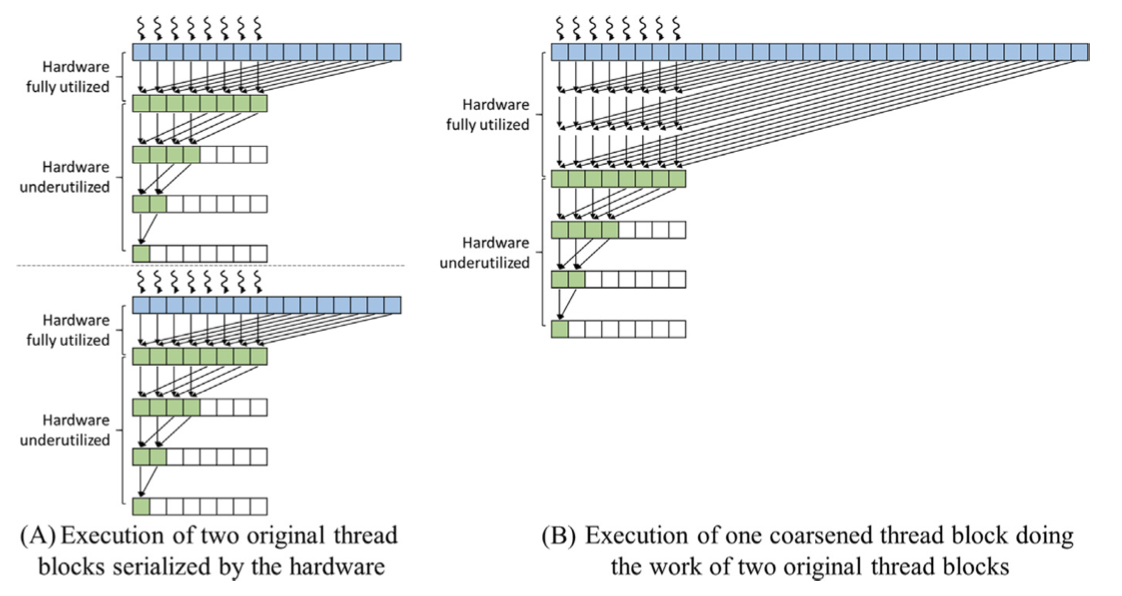
\includegraphics[width=0.9\textwidth]{figs/F10.16.png}
	\caption{\textit{比较有和没有线程粗化的并行归约。}}
\end{figure}

图 10.16 比较了两个未经硬件串行粗化的原始线程块的执行情况(如图 10.16A 所示)
和一个粗化线程块执行两个线程块的工作(如图 10.16B 所示)。 
在图 10.16A 中,第一个线程块执行一个步骤,其中每个线程将其负责的两个元素相加。 
在此步骤中所有线程都处于活动状态,因此硬件得到充分利用。 
其余三个步骤执行归约树,其中每个步骤有一半线程退出,从而未充分利用硬件。 
此外,每个步骤都需要屏障同步以及对共享内存的访问。 
当第一个线程块完成后,硬件会调度第二个线程块,它遵循相同的步骤,但在不同的数据段上。 
总的来说,这两个块总共需要八个步骤,其中两个步骤充分利用硬件,六个步骤未充分利用硬件,需要屏障同步和共享内存访问。

相比之下,在图 10.16B 中,相同数量的数据仅由粗化了 2 倍的单个线程块处理。该线程块最初执行三个步骤,
其中每个线程添加其负责的四个元素 。 所有线程在所有三个步骤中都处于活动状态,因此硬件得到充分利用,
并且不会执行屏障同步或对共享内存的访问。 其余三个步骤执行归约树,其中每个步骤有一半线程退出,未充分利用硬件,
并且需要屏障同步和对共享内存的访问。 总的来说,只需要六个步骤(而不是八个),其中三个步骤(而不是两个)充分利用硬件,
另外三个步骤(而不是六个)未充分利用硬件,需要屏障同步和共享内存访问。 
因此,线程粗化有效地减少了硬件未充分利用、同步和共享内存访问带来的开销。

理论上,我们可以将粗化因子增加到远远超过 2。 然而,必须记住,当我们粗化线程时,并行完成的工作就会减少。 
因此,增加粗化因子将减少硬件利用的数据并行量。 
如果我们将粗化因子增加太多,以致我们启动的线程块少于硬件能够执行的线程块,我们将不再能够充分利用并行硬件执行资源。 
最佳粗化因子可确保有足够的线程块来充分利用硬件,这通常取决于输入的总大小以及特定设备的特性。

\subsection{总结}
并行归约模式很重要,因为它在许多数据处理应用程序中起着关键作用。 尽管顺序代码很简单,但读者应该清楚,需要多种技术来实现,
例如用于减少发散的线程索引分配、使用共享内存来减少全局内存访问、使用原子操作进行分段减少以及线程粗化。 大输入的高性能。 
归约计算也是前缀和模式的重要基础,前缀和模式是并行化许多应用程序的重要算法组件,并且将是第 11 章“前缀和(扫描)”的主题。